\section{Automatische Verfahren zur Prädiktorauswahl}
Zu Beginn der psychologischen Forschung mussten Modelle von Hand berechnet werden. Zwangsläufig wurden wenige Prädiktoren erhoben und einfache Modelle gerechnet. 
Friedman analysierte beispielsweise 1944 die Langlebigkeit von Turbinenschaufeln in Abhängigkeit von Stress, Temperatur und einigen Legierungsparametern. 
Zwar wurde die Berechnung nicht mehr von Hand durchgeführt, doch benötigte eine Regressionsschätzung inklusive Berechnung der Teststatistiken rund 40 Stunden \cite[p.2]{armstrong2011illusions}. Jeder durchschnittliche Computer erledigt dies heutzutage in Sekundenbruchteilen. 
Mit dem technischen Fortschritt einhergehend wurden Verfahren entwickelt, welche alle möglichen Kombinationen von Prädiktoren, inklusive ihrer Interaktionen, berücksichtigen und gegeneinander testen.

Es gilt also, das ``beste'' Modell zu schätzen. 
Gemeint ist mit dem ``besten'' Modell das, das innerhalb des Trainingsdatensatzes die beste Vorhersage liefert. 
Anhand des Trainingsdatensatzes wurde das Modell jedoch auch geschätzt. Entsprechend kann es Modelle geben, die in der Gesamtpopulation bessere Vorhersagen liefern. 
``All models are wrong, but some are useful'' \cite[p.202]{box1979robustness}.
Box will damit hervorheben, dass obschon in der Literatur oft vom ``besten'' oder ``wahren'' Modell gesprochen wird, dies nur eine Approximation der Wirklichkeit darstellt \cite[p.172]{weakliem2004introduction}.

\subsection{Exhaustive Schätzung} 
Eine naive Herangehensweise ist, alle möglichen Modelle, welche mit $p$ Prädiktoren möglich sind, durchzurechnen. 
Zur Beurteilung der Modellgüte kann die mittlere quadratische Abweichung herangezogen werden.
Das Modell mit der kleinsten Fehlerquadratsumme $SSE_p$ wird als das  optimale Modell bezeichnet \cite[p. 6]{thompson1978selection}. 

\begin{equation}
SSE_p = \sum_{i=1}^n(y_{ip}-\hat y_{p})^2
\tag{Fehlerquadratsumme}
\end{equation}


Da alle möglichen Kombinationen durchgerechnet werden, wird das  Modell gefunden, das den Trainingsdatensatz am besten vorhersagt.
\citeA[p.6]{thompson1978selection} sieht einzig den Nachteil darin, dass der \Gls{glos:rechenaufwand} exponentiell mit der Anzahl zu berücksichtigender Prädiktoren steigt. 
Es müssen immer $2^p-1$ Modelle berechnet werden, bei 5 Prädiktoren sind dies 31 Modelle, bei 10 bereits 1023 usw.
Während früher eingeschränkte Rechenkapazität oft ein ökonomischer Faktor war -- es musste Rechenzeit in einem Rechenzentrum reserviert werden -- spielt die Rechengeschwindigkeit auf modernen Systemen eine untergeordnete Rolle. 
%In der psychologischen Forschung muss oft nur eine Handvoll Prädiktoren in die Schätzung einbezogen werden.

\subsection{Schrittweise Verfahren} 
Das optimale Modell beinhaltet jeden Prädiktor, der die Voraussage auch nur minimal verbessert. 
Es stellt sich die Frage ob diese minimale Verbesserung auch nützlich ist oder einfach durch Zufall entstanden ist. 
Schrittweise Verfahren arbeiten wesentlich liberaler.  Prädiktoren werden hinzugefügt oder eliminiert, je nach deren Relevanz für die Modellgüte. 
Es werden Kriterien festgelegt, nach welchen ein Modell als angemessen zu betrachten ist. 
Dies hat gegenüber dem \gls{glos:exhaustive Verfahren} den Vorteil, dass nicht alle Modelle berechnet werden müssen und entsprechend schneller Lösungen gefunden werden.

Innerhalb der schrittweisen Verfahren unterscheidet man zwischen \textit{Forward Selection} und \textit{Backward Elimination}. 
\begin{figure}[H]
	\centering
	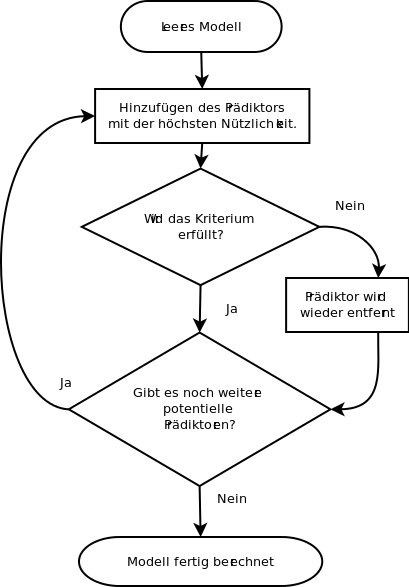
\includegraphics[height=0.5\textheight]{forward_stepwise.png}
	\caption{Forward Selection. Das Flussdiagramm beschreibt den schrittweisen Aufbau eines neuen Modells aus dem leeren Modell durch Hinzufügen potentieller Prädiktoren.}
	\label{fig:forward_stepwise}
\end{figure}
Ausgehend vom leeren Modell werden in der ersten Variante schrittweise weitere Variablen der Nützlichkeit nach in das Modell integriert. Dies dauert so lange an, bis kein Prädiktor mehr gefunden wird, der ein gewisses Kriterium erfüllt.
\begin{figure}[H]
	\centering
	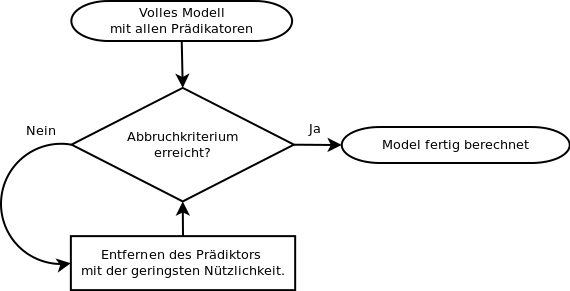
\includegraphics[height=0.5\textheight]{backward_stepwise.png}
	\caption{Backward Elimination. Das Flussdiagramm beschreibt die schrittweise Elimination von unnützen Prädiktoren aus dem vollen Modell.}
	\label{fig:backward_stepwise}
\end{figure}
In der zweiten Variante werden alle Prädiktoren in das Modell integriert und sukzessive nacheinander entfernt. Wiederum endet das Verfahren, sobald kein Prädiktor mehr weggelassen werden kann, ohne dass ein gewisses Kriterium unterschritten wird.

Die Aufnahme einer neuen Variable kann dazu führen, dass eine bereits im Modell vorhandene Variable obsolet wird. 
Um diesem Umstand Rechnung zu tragen, werden oft Forward Selection und Backward Elimination kombiniert \cite[p. 461]{bortz2011}. 

In seltenen Fällen kann es vorkommen, dass zwei Variablen für sich in die Regressionsgleichung aufgenommen, die Vorhersage kaum verbessern und das Kriterium nicht erfüllen. Zusammen leisten sie jedoch  einen substantiellen Beitrag \cite[p.261]{jacob2003applied}. 
\Gls{glos:schrittweise Verfahren} mittels Forward Selection sind entsprechend nicht in der Lage solche Effekte mit zu berücksichtigen, wogegen Backward Elimination robuster gegen solche Spressionseffekte ist \cite{shieh2006suppression}. 

Zentrales Element der schrittweisen Regression ist das Kriterium zur Beurteilung der  Modellanpassung, welches besagt, weshalb und wann ein Modell als akzeptabel zu betrachten ist. Als Folge dessen wird damit auch die Anzahl relevanter Prädiktoren bestimmt. Im Laufe der Zeit wurden diverse Kriterien definiert, welche alle für sich ihre Berechtigung haben.
Einteilen lassen sie sich in Kriterien, welche (a) sich auf die Beurteilung innerhalb des Trainingsdatensatzes beschränken oder (b) die Generalisierbarkeit ausserhalb des Trainingsdatensatzes zu berücksichtigen versuchen. Letztere werden im Abschnitt des Overfittings beschrieben.

Interessiert uns die \Gls{glos:Modellguete} innerhalb des Trainingsdatensatzes bietet das Bestimmtheitsmass erste Hinweise. Im Fall der multiplen Regression entspricht dies dem Quadrat des multiplen Korrelationskoeffizienten $R^2$ und  besagt wie viel systematische Varianz durch das Modell aufgeklärt  wird. 
Das Bestimmtheitsmass steigt mit der Anzahl der Prädiktoren $p$, insbesondere bei kleinem Stichprobenumfang $n$, weshalb eine Schrumpfungskorrektur vorgenommen werden muss \cite[p. 451]{bortz2011}. 

\begin{equation}
\bar R^2=1-\frac{\displaystyle \frac{1}{n-p-1} \sum_{i=1}^n (Y_i-\hat{Y}_i)^2}{\displaystyle \frac{1}{n-1} \sum_{i=1}^n (Y_i-\bar{Y})^2}
\tag{korrigiertes Bestimmtheitsmass}
\end{equation}

In schrittweisen Verfahren wird nicht einzig aufgrund von $R^2$ selektiert sondern es wird zusätzlich getestet, ob Verbesserungen nicht durch Zufall entstanden sind. 

Beim Signifikanztest als Kriterium wird das Verfahren beendet, wenn kein Prädiktor mehr hinzugefügt werden kann, der das Vorhersagepotential signifikant erhöht \cite[p.48]{bendel1977comparison}. 
Das Vergleichen zweier Regressionsgleichungen mittels Signifikanztest bedingt, dass diese geschachtelt sein müssen, das kleinere Modell muss im grösseren enthalten sein \cite[p. 508]{jacob2003applied}.
Das gewählte Signifikanzniveau ist eigentlich unbegründet gewählt \cite[p. 174]{weakliem2004introduction}. \citeA[p. 269]{derksen2011backward} diskutieren mehrere Empfehlungen für Signifikanzniveaus und weisen darauf hin, das sich über mehrere Tests der $\alpha$-Fehler kumuliert. 
In  Simulationen mit artifiziellen Daten zeigen \citeA{mundry2009stepwise} das  Problem multipler Tests beispielhaft auf. 
Daraus resultierend lehnen sie die Verwendung der schrittweisen Regression mittels Signifikanztest gar ab.

Ein weitere Schwäche des Hypothesentestens ist der Einfluss der Stichprobengrösse. So kann bei genügend grossem Umfang nahezu jedes Modell  signifikant werden, was wiederum zu komplexen und überangepassten Modellen führt \cite[p.173]{weakliem2004introduction}.

Entgegen dem exhaustiven Verfahren besteht bei Schrittweisen das Problem, dass unter Umständen nicht das optimale Modell gefunden wird. 
\citeA[p. 462]{bortz2011} bezeichnen diese Verfahren eher als explorativ, da die Nützlichkeitsunterschiede, welche oft nur geringe statistische Bedeutung haben, das Modell bestimmen.
\citeA[p. 56ff]{harrell2001regression} lehnt das Verfahren gar ab und führt ins Feld, dass sämtliche statistischen Prinzipien verletzt würden. 
\citeA{berk1978comparing} zeigte jedoch in einem Vergleich, dass die durchschnittliche Differenz der Fehlerquadratsummen zwischen exhaustiven und schrittweiser Regression kaum 7\% übertrifft. 